%%=============================================================================
%% Elasticsearch en X-Pack
%%=============================================================================

\chapter{Elasticsearch en X-Pack}
\label{ch:elasticsearch-xpack}


Elasticsearch is het hart van elastic stack. Het is de databank die alle JSON-elementen bevat die reeds gemaakt werden door Logstash. 
Het bevat een geavanceerd zoekalgoritme gebaseerd op indices. Voor een hoeveelheid data onder duizend elementen wordt beter iets anders gebruikt aangezien de start tijd van Elasticsearch enkele seconden bedraagt.
Maar voor enkel miljoenen elementen is het zeer geschikt. Na de starttijd kan Elasticsearch zo goed als live de zoekopdrachten volbrengen. 
Omwille van de uitermate goede schaalbaarheid wordt het reeds bij enkele bedrijven gebruikt die met heel veel data af te rekenen krijgen \autocite{15companies}.

Om Elasticsearch optimaal te laten werken, is het zeer belangrijk om juist om te gaan met indices. Als voorbeeld gezocht wil worden op een bepaalde dag van de week dan kan hiervoor best een afzonderlijk field voorzien worden. 
Daarom is het dus erg belangrijk om werk te maken van het schrijven van een goede config file voor logstash.

Het gebruik van de zelf ontwikkelde taal is niet eenvoudig en daarom zal in \ref{sec:search} enkele basis mogelijkheden toegelicht worden.
De commando's kunnen via de console in Kibana gerund worden of via de commandline. In de rest van de bachelorproef zullen de stukken code gebruikt worden voor in de console van Kibana.
Indien gewenst kunnen deze stukken code ook gebruikt worden in de commandline, maar dan wel in combinatie met curl.

X-Pack is een recente uitbreiding op de elastic stack. Deze tools groeien erg snel en er komen er nog steeds bij. 
Deze tools zijn gebasseerd op het sterk algoritme van Elasticsearch. 

\section{Search}
\label{sec:search}

Elasticsearch is eerst en vooral een database en daar horen natuurlijk zoekopdrachten bij. Elasticsearch werkt niet met sql queries, maar heeft daar een eigen taal voor. Er zijn twee soorten zoekopdrachten:
\begin{itemize}
	\item \textbf{Leaf query: } dit zoekt voor specifieke waarden in bepaalde fields, dit door queries zoals match, term, range. Deze queries kunnen afzonderlijk gebruikt worden.

	\item \textbf{Compound query: } deze queries combineren leaf of andere compound queries op een logische manier (zoals met bool of dis\_max).
\end{itemize}

In onderstaand stuk code worden leaf queries samengebracht tot één compound query. Eerst en vooral zal een filter uitgevoerd worden die ervoor zorgt dat de rest alleen uitgevoerd zal worden op een beperkte selectie elementen.
In dit voorbeeld zal enkel gewerkt worden op elementen die backup als user hebben.
Als tweede deel zal gezocht worden naar een element dat "drop table" bevat. 
Deze zoekopdrachten werden uitvoerd op de elementen met de index linux.


\lstset{escapechar=@,style=customc}  
\begin{lstlisting}[frame=single]  
POST /linux
{
    "query": {
        "bool" : {
            "must" : {
                "query_string" : {
                    "query" : "drop table",
                }
            },
            "filter" : {
                "term" : { "user" : "backup" }
            }
        }
    }
}
\end{lstlisting}

Er zijn nog heel wat mogelijkheden en deze zijn terug te vinden in de documentatie. 
Zoekopdrachten kunnen nuttig zijn in het zoeken naar een probleem. Maar voor het monitoren is dit minder van toepassing.
De toepassingen die als volgende besproken worden, maken hier in de achtergrond natuurlijk wel gebruik van.

\section{Watcher}
\label{sec:watcher}

Watcher is één van de tools die tot de Elastic stack behoren. Het kijkt uit naar veranderingen of anomalieën in de data en voert de nodige vervolgacties uit \autocite{watherdynamic}. Er zijn enkele belangrijke eigenschappen nodig om watcher te kunnen gebruiken:
\begin{itemize}
	\item de relavante data of data verandering kan periodiek opgevraagd worden met een query,
   
   \item de resultaten van de query kunnen gematcht worden aan de voorwaarden,

	\item één of meerdere acties worden ondernomen als de voorwaarden voldaan zijn.
\end{itemize}

Een Watch query bestaat uit vier delen: planning, zoekopdracht, conditie en actie. 
\begin{itemize}
	\item \textbf{Planning: } een planning voor het laten lopen van een zoekopdracht en het checken van de conditie.
   
    \item \textbf{Zoekopdrach: } de zoekopdracht is de input voor de conditie. Het ondersteunt de volledige elasticsearch. 

	\item \textbf{Conditie: } is een conditie die beslist wanneer er acties moeten volgen. Het is mogelijk hier te werken met true or false maar ook het schrijven van meerdere scenarios is toegestaan.
    
    \item \textbf{Actie: } een e-mail zenden, 3rd party software waarschuwen, de opgevraagde data stockeren, \dots.
\end{itemize}

Dit is dus ook een erg belangrijke tool voor het monitoren.
Watcher zal gebruikt worden om duidelijke boodschappen te e-mailen van waar zich een probleem voor doet.
Dit is ook de tool die gebruikt moet worden om alerts te voorzien bij het gebruik van grafieken of andere tools.

\section{Shield}
\label{sec:shield}

Shield maakt het mogelijk op een eenvoudige manier de Elastic stack te beveiligen. Met het gebruik van Shield wordt alle data pas vrijgegeven na het inloggen met gebruikersnaam en paswoord. Dit zorgt ervoor dat niemand met slechte bedoelingen zo maar aan de data zou kunnen. 
Maar tegenwoordig zijn er al andere manieren om die data toch te kunnen bemachtigen. Daarom zijn er ook meer geavanceerde mogelijkheden zoals:
\begin{itemize}
	\item data-encryptie voor communicatie tussen de nodes,
    
    \item  beperkte toegang voor bepaalde users,

	\item IP-filtering.
\end{itemize}

In shield zit ook een module die zorgt voor data integriteit. Het bevat een eigen protocol dat de data zal encrypten tussen de nodes en daarna nog een authenticatie bericht zal zenden. Dit zorgt er voor dat er geen foute data of een tekort aan data zal ontstaan.

Indien shield geïmplementeerd wordt, dienen ook de config files in logstash aangepast worden. Deze moeten dan voorzien worden van een gebruikersnaam en paswoord.

\section{Monitoring}
\label{sec:monitoring}

Deze monitoring tool maakt het mogelijk om via Kibana de volledige Elastic stack te monitoren. Onder dit monitoren wordt verstaan het bekijken van de preformance van de Elastic stack in realtime.
Er wordt een agent geïnstalleerd die uit alle nodes metrtics gaat verzamelen.
Deze data worden dan verwerkt en zal aan de hand van een dashboard de prestaties van de Elastic stack weergeven. 
Het kijkt naar de prestaties zoals hoelang zoekopdrachten duren in Elasticsearch. Hier wordt ook nog systeeminformatie gegeven. Dingen zoals geheugen gebruik, aantal gebruikte shards, uptime, \dots \autocite{clusterstatus}.

\section{Machine learning}
\label{sec:machine-learning}

Deze tool kwam uit in 5.4 en was nog in beta maar werd met zicht op de casus toch opgenomen \autocite{machinelearningdemo}.
Bij Machine Learning draait het er om dat de machine slimmer wordt en gaat herkennen wanneer zich een anomalie voor doet. Hoe meer input data hoe beter het onregelmatigheden zal gaan herkennen.
Het berekent een beneden- en bovenlimiet. Afhankelijk van de afwijking daarvan zal een anomalie score berekend worden. Deze scores worden dan nog eens in vier categorieën opgedeeld. 
Dan kan gekozen worden op welk van de vier categorieën gealert wordt en op welke niet.
\begin{figure}[h]
	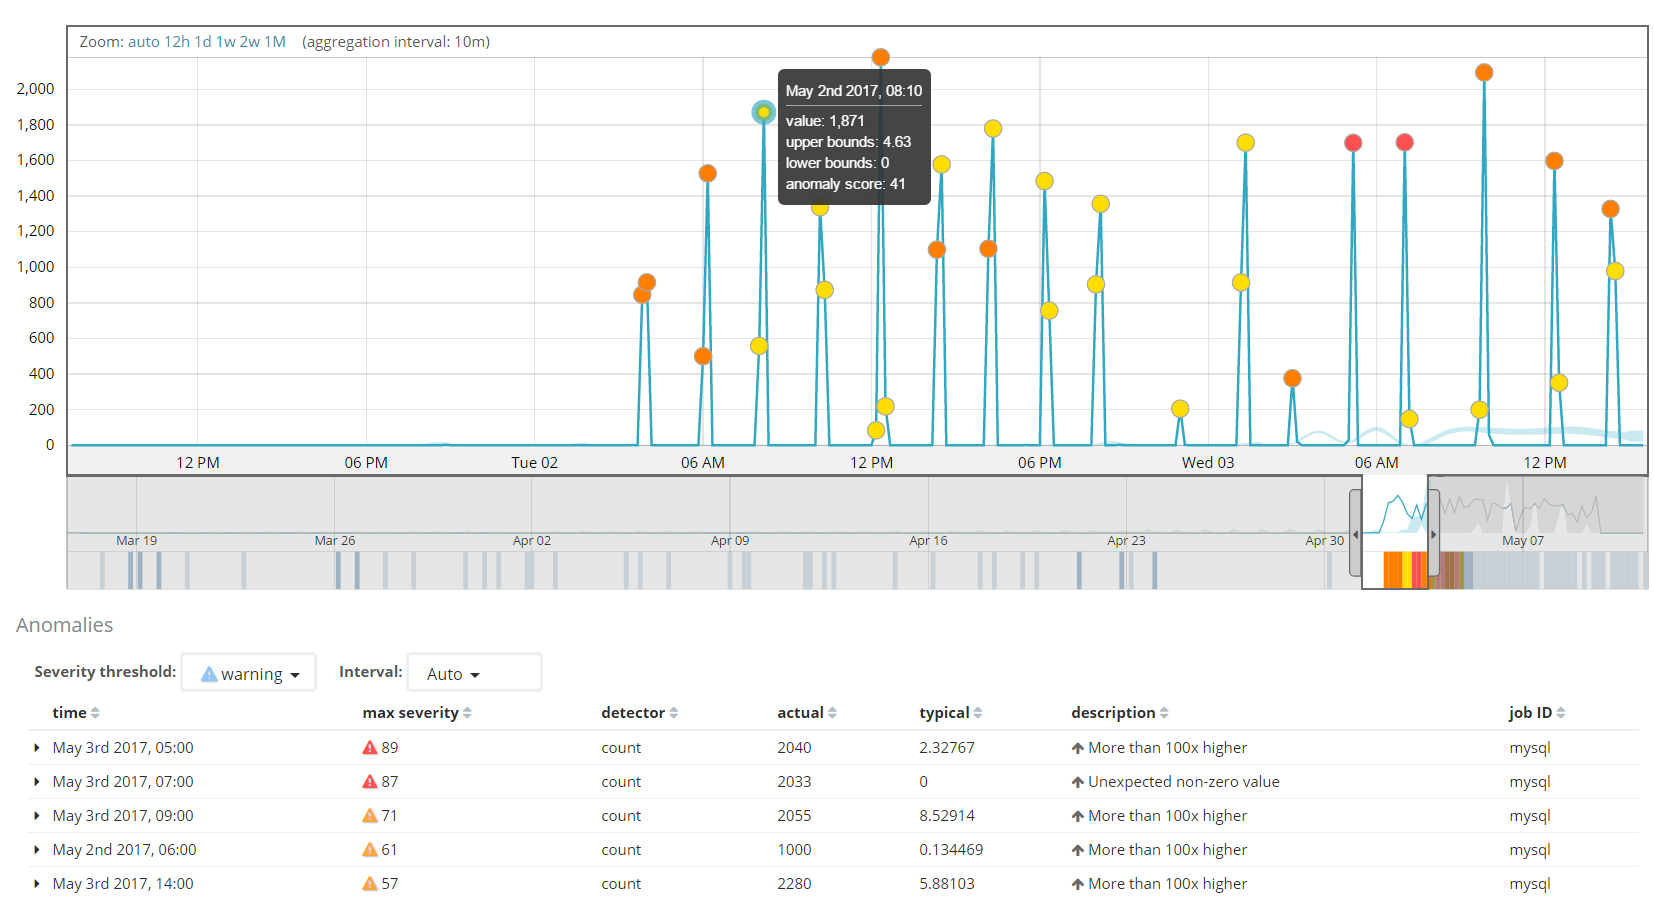
\includegraphics[width=16cm]{img/machinelearning1}
	\caption{Machine Learning toegepast op de hoeveelheid loglijnen gecreëerd door een MSSQL.}
	\label{fig:machinelearning1}
\end{figure}

Er kan ook een vergelijking gemaakt worden tussen verschillende reeksen binnen Machine Learning om te zien als er een verband bestaat tussen hen. 
Dit kan ervoor zorgen dat de bron van een probleem sneller gevonden kan worden.
\begin{figure}[h]
	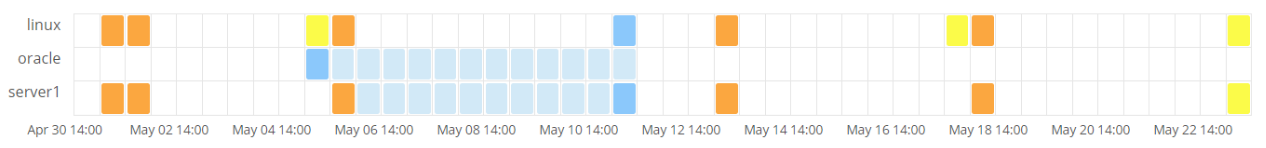
\includegraphics[width=10cm]{img/machinelearning2}
	\caption{Overzicht van anomalieën bij: Server}
	\label{fig:machinelearning2}
\end{figure}
